\documentclass[12pt]{article}
\usepackage{amsmath,amssymb,amsthm}
\usepackage{fullpage}
\usepackage{graphicx}
\usepackage{hyperref}
\usepackage{url}
\usepackage{booktabs}

\theoremstyle{definition}
\newtheorem{thm}{Theorem}[section]
\newtheorem{lem}[thm]{Lemma}
\newtheorem{corr}[thm]{Corrolary}
\newtheorem{defn}{Definition}[section]
\newtheorem{conj}{Conjecture}[section]
\newtheorem{prob}{Open problem}[section]
\newcommand{\floor}[1]{\left\lfloor #1 \right\rfloor}
\newcommand{\ceil}[1]{\left\lceil #1 \right\rceil}
\newcommand{\bigC}[0]{\mathcal{C}}
\begin{document}
\emergencystretch 3em
\title{A lower bound from a random walk? (DRAFT)}

\author{Josh Burdick}

\maketitle

\begin{abstract}
The study of random walks on graphs has a long history (FIXME make this less vague).
Here, we define a random walk, and try to use it to
give a lower bound on CLIQUE.
\end{abstract}

\newpage

\tableofcontents

\vspace{5mm}


\section{A Counting Bound} \label{se:countingBound}

Previously, we considered the set of functions BUGGYCLIQUE, which
only detect a subset of the possible cliques \cite{buggyclique}.
Using a slight modification of Shannon's
function-counting argument \cite{shannon_synthesis_1949},
we showed that a function randomly chosen from BUGGYCLIQUE,
on average, requires $\Omega(n^{k/2})$ two-input NAND gates to compute.

\subsection{A random walk on the zeroing-out lattice}

Previously, we defined the zeroing-out lattice $Z$, in which all paths lead
``down`` to $\emptyset$. Here, we consider a ``bouncing'' walk
through $Z$, starting from an arbitrary set of cliques $A_t$.

\begin{enumerate}

\item Feed in a 0 to a randomly-chosen edge $e$ of $C(A_t)$. 
This corresponds to
following a random arc ``down''. Call the resulting set $B_t$ (
for ``bounce'').

\item Add a random set of the possible cliques which include $e$,
resulting in a larger set $A_{t+1}$. This corresponds to following
a random arc ``up''.

\item Repeat...

\end{enumerate}

One step of this is depicted in Figure \ref{fig:boing}.

Luca Trevisan's blog discussed ways of understanding a hypergraph by
considering a random walk on a related graph
\cite{luca_trevisan_blog_random_walks_1}.
What we discuss here is different, but seems somewhat related:
we are looking at a random walk on a graph whose vertices are
hypergraphs.

\begin{figure}

\centering

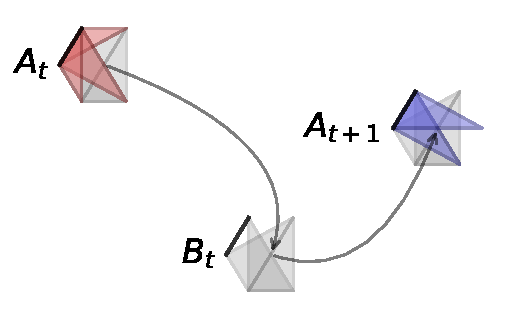
\includegraphics[width=0.5\textwidth]{bounce.pdf}

\caption{
One step of the walk. Starting from $A_t$, the cliques containing 
to a randomly-chosen edge are removed, resulting in $B_t$.
Adding a random set of cliques back results in $A_{t+1}$.
}
\label{fig:boing}

\end{figure}

\subsection{Graph-theoretic properties of the walk}
Note that ``one-step reachability'' in the bouncing walk is symmetric;
one step can be an arbitrary modification of which cliques which hit
an edge $e$ are included.
Thus, we can construct a new undirected graph, $S$, with an edge between every
pair of sets of cliques reachable in one step.

\begin{defn} \label{def:bouncingWalk}

Let $Z$ be the previously-defined zeroing-out graph. We will write $Z'$ for
the inverse of that graph (with arrows reversed).

The bouncing walk $S$ is result of following one edge of $Z$, followed by one
edge of $Z'$. Formally, as a relation:

\[
S(a,c) \triangleq \exists b. Z(a,b) \land Z'(b,c)
\]

\end{defn}

We can also characterize $S$ by XORing sets of cliques together.

\begin{defn} \label{def:oneEdgeNeighbors}

Let $A$ be a set of cliques, and let $e$ be an input edge. We write
$e \subset A$ if some clique in $A$ contains the edge $e$.

We define the set of one-edge neighbors $E$, as follows:

\[
E = \emptyset \cup \bigcup_e \{ X: e \subset X\}
\]

\end{defn}

For any given set of cliques $A$, we can generate all the neighbors
of $A$ by picking a set of cliques $X \in E$, and taking $A \oplus X$. This will
add and remove some cliques from $A$, all of which include some edge $e$.
Distinct choices of $X$ will yield distinct neighbors of $A$.
We can enumerate these by picking an edge $e$, 
and then picking any subset of cliques which contains $e$. (This overcounts
elements in $E$, but not by that much; most random sets of cliques won't be
covered by a single edge $e$.) Thus, we have the following bounds for $|E|$:

\[
2^{{n-2} \choose {k-2}} \le |E| \le {n \choose 2} 2^{{n-2} \choose {k-2}}
\]

XORing with something from $E$ defines all of the neighbors of any set of cliques
(FIXME reword this).
Thus, we get that $S$ is a $d$-regular graph, with $d = |E|-1$.
I'm not sure if it's a known $d$-regular graph.
It seems too
dense to be an expander, but does seem to be pretty strongly connected.

\subsection{Modelling where the walk goes}

We have two steps, in which cliques are first removed, then added.
We denote transition matrices for these two steps by $L$ and $U$, respectively.
As before, let $N = {n \choose k}$.
We also define the number of cliques which potentially could be ``hit'' by
zeroing out an edge as $h = {{n-2} \choose {k-2}}$.

In the first step, when edge $e$ is zeroed out, the number of cliques removed has
a hypergeometric distribution. (This is because $|A_t|$ of the $N$ possible cliques
are present, and we're ``hitting'' $h$ of those when we zero out $e$.)

\[
|A_t - B_t| \sim \text{Hypergeometric}(N, |A_t|, h)
\]

In the second step, we know that {\em no} cliques contain $e$. The number of
cliques we might add (each chosen uniformly with probability 0.5) has 
a binomial distribution. We have that

\[
|A_{t+1} - B_t| \sim \text{Binomial}(h, 2)
\]

We now write $L$ and $U$ for the $n=5, k=3$.

\begin{verbatim}
L =
[[1.    0.    0.    0.    0.    0.    0.    0.   ]
 [0.3   0.7   0.    0.    0.    0.    0.    0.   ]
 [0.067 0.467 0.467 0.    0.    0.    0.    0.   ]
 [0.008 0.175 0.525 0.292 0.    0.    0.    0.   ]
 [0.    0.033 0.3   0.5   0.167 0.    0.    0.   ]
 [0.    0.    0.083 0.417 0.417 0.083 0.    0.   ]
 [0.    0.    0.    0.167 0.5   0.3   0.033 0.   ]
 [0.    0.    0.    0.    0.292 0.525 0.175 0.008]
 [0.    0.    0.    0.    0.    0.467 0.467 0.067]
 [0.    0.    0.    0.    0.    0.    0.7   0.3  ]
 [0.    0.    0.    0.    0.    0.    0.    1.   ]]

U =
[[0.125 0.375 0.375 0.125 0.    0.    0.    0.    0.    0.    0.   ]
 [0.    0.125 0.375 0.375 0.125 0.    0.    0.    0.    0.    0.   ]
 [0.    0.    0.125 0.375 0.375 0.125 0.    0.    0.    0.    0.   ]
 [0.    0.    0.    0.125 0.375 0.375 0.125 0.    0.    0.    0.   ]
 [0.    0.    0.    0.    0.125 0.375 0.375 0.125 0.    0.    0.   ]
 [0.    0.    0.    0.    0.    0.125 0.375 0.375 0.125 0.    0.   ]
 [0.    0.    0.    0.    0.    0.    0.125 0.375 0.375 0.125 0.   ]
 [0.    0.    0.    0.    0.    0.    0.    0.125 0.375 0.375 0.125]]
\end{verbatim}

We let $S = LU$ be the transition probability after both of these steps.
If we pick a set of cliques $A$ uniformly at random,
then the number of cliques, $|A|$, has a binomial distribution.
We can check that this distribution
is the stationary distribution of $S$:

\begin{verbatim}
binomial coefficients x =
[  1  10  45 120 210 252 210 120  45  10   1]

x * L * U =
[  1.  10.  45. 120. 210. 252. 210. 120.  45.  10.   1.]
\end{verbatim}

\section{A bound using integer programming?}

We now attempt to obtain a bound on CLIQUE from this random walk, by
writing what we know as a mixed integer program (IP), and then bounding it
using the LP relaxation. Previously, we used an LP \cite{buggyclique}.
(Alternatively, we could solve the IP; however, that seems likely to
be computationally difficult and/or complicated.)

(FIXME variable names may need re-thinking; I don't know what
conventions are common in stating integer programs.)

\subsection{Variables and objective function}

First, for a given $n$ and $k$, let $N = {n \choose k}$; this is
the maximum possible number of cliques.

We choose a maximum number of gates $G$ to consider. (If $G$ is
chosen too small, then the problem will be infeasible.)

Then, for $0 \le c \le N$ and $0 \le g \le G$,
we define an integer variable $w_{c,g}$ be the number of functions which contain
exactly $c$ of the possible $N$ cliques, and which require at least
$g$ gates to detect. ($w$ might be considered short for ``weight?'';
it's essentially histogram counts.)

We also define a real-valued variable
$x_c$ as ``expected number of gates needed, for sets of size $c$'':

\[
x_c = \sum_g g \cdot w_{c,g}
\]

Our question: how many gates are in the smallest circuit
which detects {\em all} the cliques? Thus, the objective function
is

\[
\text{Minimize }x_N\text{, subject to the constraints...}
\]

Next, we state the constraints.

\subsection{Counting functions}

Let $m = {n \choose 2}$ be the number of inputs; that is the number
of input edges for an $n$-vertex graph.

We have the counting argument: the number of $m$-input functions
constructable using $g$ gates is bounded. (This number increases
quickly as a function of $g$, but nonetheless is bounded.)

\[
\sum_c w_{c,g} \le \text{some fast-growing function of }g
\]

FIXME include table of these numbers for, e.g., 6-input circuits,
for $1 \le g \le 5$.

We might think of the set of functions as filling a conical
martini glass. If we consider the $z$ axis to be ``number of gates'',
then there is ``room for more functions higher up.''

\subsection{Counting sets of cliques}

We also know the number of sets of cliques (and thus, the number
of BUGGYCLIQUE functions) for a given number of cliques $c$.

\[
\sum_g w_{c,g} = {N \choose c}
\]

Note that this has a sharp maximal peak at $c = N/2$.

\subsection{The walking bound}

We now consider how the number of sets ($|A_t|$), and
the number of gates needed to detect them ($|C_{A_t}|$),
vary, with each step.

We only consider using unbounded fan-in NAND gates.
This is because adding one such NAND gate suffices to detect an
addtional clique, and we frequently will need to construct circuits which detect
some additional cliques.
Although unbounded-fan-in circuits have been studied
\cite{wegener1991complexity}\cite{allender1994depth}, various sorts of 2-input gates are arguably
more frequently used in circuit complexity. (Many of the results here
seem adaptable to work with 2-input gates.)

First, what can we say about $|A_t|$, the number of sets?
Consider a given starting set, $A_t$.
After a step ``down'' (with $N$ and $h$ defined as before),
the expected change in the number of cliques is:

\[
E[|A_t - B_t|] = \frac{|A_t|}{N}h
\]

After a ``bounce'' up, the corresponding expected change is:

\[
E[|A_{t+1} - B_t|] = \frac{1}{2}h
\]

What about the number of gates, $|C_{A_t}|$? For this quantity,
the situation is murkier.

On the ``down'' step, some number of gates might be eliminated.
If $A$ is large enough, then we're likely to hit at least one gate,
but for simplicity, we don't assume that this happens.
We know, however, that we didn't eliminate more than $|A_t - B_t|$
gates. (If we had, then we could construct a smaller $C_{A_t}$,
by starting with $C_{B_t}$, and ORing it with $|A_t - B_t|$
NAND gates.)

On the ``up'' step, somewhat symmetrically, we probably will
need more gates. However, we definitely can get away with
adding $|A_{t+1} - B_t|$ NAND gates to $C_{B_t}$.

Combining all of these, we have the following bounds on how much the
expected number of gates fluctuates, at each step of the random walk:

\[
-\frac{i}{N}h \le E[ |C_{A_{t+1}}| - |C_{A_t}| | |A_t|=i ] \le \frac{1}{2}h
\]

Intuitively, this suggests that the number
of gates needed is a somewhat ``smooth'' function of the
number of cliques in the circuit.

This isn't a very sharp bound. However, it applies across the entire
range of $i$, from 0 to $N$. Also, for fixed $k$, as $n$ increases,
it gets sharper.

For each possible initial number of cliques $i$, with $0 \le i \le N$,
we can use the transition matrix $S$ to express this change in the
number of gates. We then add upper and lower bounds for that $i$.

\[
E[ |C_{A_{t+1}}| - |C_{A_t}| | |A_t|=i ] = (\sum_j S_{ij} x_j) - x_i
\]

\subsection{Bound on finding zero cliques}

We also have a slightly comical upper bound:
to detect zero cliques, we simply always
output a 0. We can implement this with one NAND gate (or possibly zero;
I'm not quite sure how to count this). (We refer to this as the
``no cliques'' constraint.) We have:

\[
x_0 = 1
\]

Why might we think that this is even {\em remotely} useful? We are, after
all, trying to bound $x_N$...

Well, we know that if we start at $c=0$, if a random walk takes us to
$c \approx N/2$, then at that point, the counting bound implies that
(on average), we'll need a large-ish number of gates to detect those $c$ cliques.
The walking bound limits how much the number of gates can fluctuate
in getting there. Thus, forcing $x_0=1$ ``drags down'' the lower half of $Z$.

My intuition is that functions with smaller numbers for $c$ would
tend to ``fill up'' the space available for functions with smaller numbers of gates.
(Recall that using fewer gates, there isn't much ``space'' for many functions.)
Hopefully this would ``rule out'' things in the upper half of $Z$ (such as CLIQUE)
from having a small number of gates.

\section{Results}

Results so far are {\em incredibly} preliminary. We bound $x_N$
(that is, the expected number of gates needed to find all the cliques),
using the LP relaxation of the IP. We have tried using several
LP solvers which support exact rational solutions,
including SCIP, a pure-Python package called {\tt flexible\_lp},
and the GNU Linear Programming Kit (GLPK). Results here are
using GLPK. Thus far, we have only considered unbounded-fan-in
NAND gates.

Note that unlike previous related bounds, here we {\em only} solve minimizing
$x_N$, and plot the resulting bounds $x_j$, at that solution. The
goal here is to see what the LP considers a possible scenario, when
minimizing the number of gates for CLIQUE.

\begin{figure}

\centering

\includegraphics[width=0.8\textwidth]{bounds\_7\_3\_3.pdf}

\caption{
Bounds with $n=7$ and $k=3$, including different sets of constraints.
Note that this plot shows results for all the variables, when
minimizing $x_N$.
}
\label{fig:bounds0}

\end{figure}

Figure \ref{fig:bounds0} shows results thus far.
Parts of this plot make sense. For instance, when the
step and ``no cliques'' constraints are included, the
plot goes somewhat smoothly up from $(0,1)$. (The counting
bound is flat, but presumably this is because
that one unbounded-fan-in NAND gate, with ${5 \choose 2}$
input wires, can implement $2^{5 \choose 3}$ different
functions.)

On larger instances, the LP crashes. This seems to be because even
solvers (such as GLPK and the exact version of SOPLEX) can
theoretically can solve problems with fractions involving
numbers like $10^{100}$, in practice, these haven't worked
(for differing reasons).

More recently, I have tried to modify the Python code from
Jeremy Kun's tutorial about the simplex algorithm \cite{kun_lp_simplex}.
Although replacing double-precision with Python {\tt fractions.Fraction}
objects works, the resulting code isn't working, for this particular
problem.

This raises the following open question:

\begin{prob}
What bound would this give for CLIQUE, if the LP {\em didn't} crash?
\end{prob}

\section{Conclusion}

One appealing thing about this approach is that it gives a
bound for clique in any event. Even if the bound weren't
superpolynomial, in the unlikely event that were even superlinear,
that {\em would} be exciting.

It seems worth {\em strongly} emphasizing, then, that currently this gives a bound
of 1 unbounded fan-in NAND gate...

\section{Acknowledgements}

The emphasis on random walks was partly inspired by the late Luca Trevisan's
blog, {\em in theory};
as many complexity commentators have noted, he will be missed.
The author would also like to thank the authors and maintainers of
several other entertaining and relevant blogs, including but
not limited to: the Computational Complexity blog
(Lance Fortnow and William Gasarch),
G\"odel's Lost Letter (Richard Lipton and Ken Regan),
and Shtetl-Optimized (Scott Aaronson).

\bibliography{references}
\bibliographystyle{unsrt}

\end{document}

